\section{Numerical validation of the sampler and correlations}
\label{sec:simulation}

The theorem already establishes the reciprocal identities. The purpose of this study is narrower: to check that the bounded-window sampler and the edge-corrected estimators reproduce the analytical model at the resolution attainable by Monte Carlo. We use the single expanded-witness parameter set
\[
 \delta=h=0.49,\quad H=0.98,\quad M=36.21,\quad P=50.01\ \mathrm{km},
 \qquad a_2=10^{-13}\ \mathrm{km}^{-5}
\]
at every order. It gives
\begin{align*}
 \rho&=1.5712738489\times10^{-9}\ \mathrm{km}^{-3},
 & C_2&=4.05038434\times10^4\ \mathrm{km},\\
 C_3&=2.48998981\times10^8\ \mathrm{km}^2,
 & C_4&=5.15442831\times10^{11}\ \mathrm{km}^3.
\end{align*}
These constants are fixed from the construction; none is fitted to a numerical curve.

\subsection{Design and estimators}

We simulate independent restrictions to equal cubes, including parents outside the observation cube whose daughters can enter it. Every realisation, including empty and low-count cubes, is retained. Parent labels are stored only for sampler diagnostics and are not used by the correlation estimators. The known value of $\rho$ is used throughout the primary study.

The first diagnostic is the translation-corrected estimator of the three-dimensional $K$-function. For the present model,
\begin{equation}
 K(r)=
 \begin{cases}
 4\pi r^3/3,&0\leq r<\delta,\\
 4\pi\delta^3/3+2\pi C_2(r^2-\delta^2),&\delta\leq r\leq P,\\
 4\pi\delta^3/3+2\pi C_2(P^2-\delta^2)+4\pi(r^3-P^3)/3,&r>P.
 \end{cases}
 \label{eq:K-model}
\end{equation}
The curve follows by integrating the full pair correlation; the lower cutoff is not a hard core because points with different parents can be closer than $\delta$. Independent Poisson controls target $4\pi r^3/3$.

We then estimate the full correlations $g_2,g_3,g_4$ with the common translation correction in Appendix~\ref{app:estimators}. Bins lie wholly within their admissible domains. Each estimate is compared with the integrated reciprocal target in \eqref{eq:bin-target}, and the compensated statistics $Dg_2$, $Ag_3$ and $Vg_4$ are compared with the fixed constants above. Table~\ref{tab:frozen-design} records the complete scalar binning and the predeclared shape cuts. Here $d_{\max}$ and $d_{\min}$ are the largest and smallest simplex-edge lengths and $h_{\min}$ is the smallest vertex-to-opposite-face altitude. The orientation variable is $|\cos\theta|$, where $\theta$ is the angle between the vertical axis and the triangle normal or, at fourth order, a longest-edge axis. Each low stratum includes its cut and each high stratum is its complement within the admissible domain. Uncertainty is computed over whole independent realisations.

\begin{table}[htbp]
\centering
\footnotesize
\caption{Frozen numerical design. Scalar edges are in km, km$^2$ and km$^3$
at orders two, three and four. Every adjacent pair defines one bin.}
\label{tab:frozen-design}
\begin{tabular}{@{}lll@{}}
\toprule
Order & scalar-bin edges & shape and orientation cuts\\
\midrule
$g_2$ & \begin{tabular}[t]{@{}l@{}}
$0.49,20.4214,28.8761,35.3641,$\\
$40.8340,45.6531,50.01$
\end{tabular}
& none\\[2pt]
$g_3$ & $0,60.88,128.37,223.24,567.7507$
& \begin{tabular}[t]{@{}l@{}}
$d_{\max}=30.46$ km; $h_{\min}/d_{\max}=0.3281$;\\
$|\cos\theta|=0.5$
\end{tabular}\\[2pt]
$g_4$ & $0,114.32,219.27,465.90,5595.2478$
& \begin{tabular}[t]{@{}l@{}}
$d_{\max}=32.576$ km; $h_{\min}/d_{\max}=0.0954$;\\
$d_{\min}/d_{\max}=0.3327$; $|\cos\theta|=0.5$
\end{tabular}\\
\bottomrule
\end{tabular}
\end{table}

The $K$ grid consists of $0$, $0.245$, $0.49$ km, the multiples of
$10/3$ km from $10/3$ to $100$ km, and the support endpoint $50.01$ km.
At orders three and four, each stratum/bin volume and reciprocal integral is
defined by the integrals in Appendix~\ref{app:estimators} with the corresponding
indicator from Table~\ref{tab:frozen-design}; the independent geometric sampler
uses one million proposals in 50 blocks. Thus the plotted targets do not depend
on undocumented bin midpoints.

\subsection{Precision pilot and fixed production design}

The precision pilot is run before the production design is fixed. It measures runtime, contributing-realisation counts, tuple occupancy, the dispersion of realisation-level contributions, and the uncertainty in the independent geometric normalisers. We use a pointwise 95\% interval half-width no larger than 10\% of the target as a binwise numerical design goal for every pooled bin. This is slightly more demanding than applying the goal only to central bins. A bin that cannot meet it is retained and labelled underpowered; we do not condition on nonempty windows, switch to same-parent tuples, or alter the parameters by order.

The pilot used $10{,}000$ independent cubes of side $1200$ km, seed
$2026101901$, and $250{,}000$ independent geometric proposals at each of orders
three and four. It found $13{,}118$ admissible unordered pairs, $322$ triangles
and only four tetrahedra. The six pair bins met the 10\% pointwise precision
goal, whereas the four pooled triangle bins had relative half-widths between
$20.4\%$ and $24.4\%$. The tetrahedron pilot was plainly uninformative.

We therefore froze the production design before examining its outcomes:
$200{,}000$ independent cubes of the same size, seed $2026101903$, the pilot's
six radial bins and four area and volume bins, and one million independent
geometric proposals per higher order. Pilot scaling predicted useful pair and
triangle estimates but only about 80 admissible tetrahedra. Reaching 10\%
fourth-order precision would require a multi-million-window run, so we retained
the prescribed estimator and recorded fourth order as underpowered. A separate
Poisson control used 200 cubes of side $120$ km at intensity
$3\times10^{-5}\,\mathrm{km}^{-3}$; this deliberately higher intensity checks
the estimators rather than imitating the cluster model.

\subsection{Production results}

The production run retained all $200{,}000$ realisations, including $47{,}055$
empty cubes. Its mean count was $2.71849$, compared with the analytical mean
$2.71516$; the sample variance was $5.32744$. The estimators used every
admissible tuple, without parent labels. For diagnosis only, the saved labels
showed that the $260{,}796$ pairs included 247 two-parent pairs, the $6{,}535$
triangles included 34 two-parent triangles, and the 126 tetrahedra included
three two-parent tetrahedra. Cross-parent allocations are rare at this
intensity, but they were not removed.

\begin{table}[htbp]
\centering
\caption{Production information for the pooled correlation estimates. The
half-width is the largest pointwise 95\% Monte Carlo half-width divided by the
fixed target among the pooled raw and compensated bins.}
\label{tab:simulation-precision}
\begin{tabular}{@{}lrrrl@{}}
\toprule
Order & tuples & scalar bins & largest half-width & assessment\\
\midrule
$g_2$ & $260{,}796$ & 6 & $1.05\%$ & informative\\
$g_3$ & $6{,}535$ & 4 & $5.42\%$ & informative\\
$g_4$ & $126$ & 4 & $39.2\%$ & underpowered\\
\bottomrule
\end{tabular}
\end{table}

The $K$-function follows the analytical curve from the first estimable radius,
$3.33$ km, through $100$ km; the model curve lies in every corresponding
pointwise interval. At $0.245$ and $0.49$ km no pair was observed. The resulting
zero empirical variance is no evidence of precision: at this intensity the
different-parent contribution below the pair support is too rare to estimate.
The higher-intensity Poisson control tracks $4\pi r^3/3$ and supplies the
small-radius implementation check.

\begin{figure}[htbp]
 \centering
 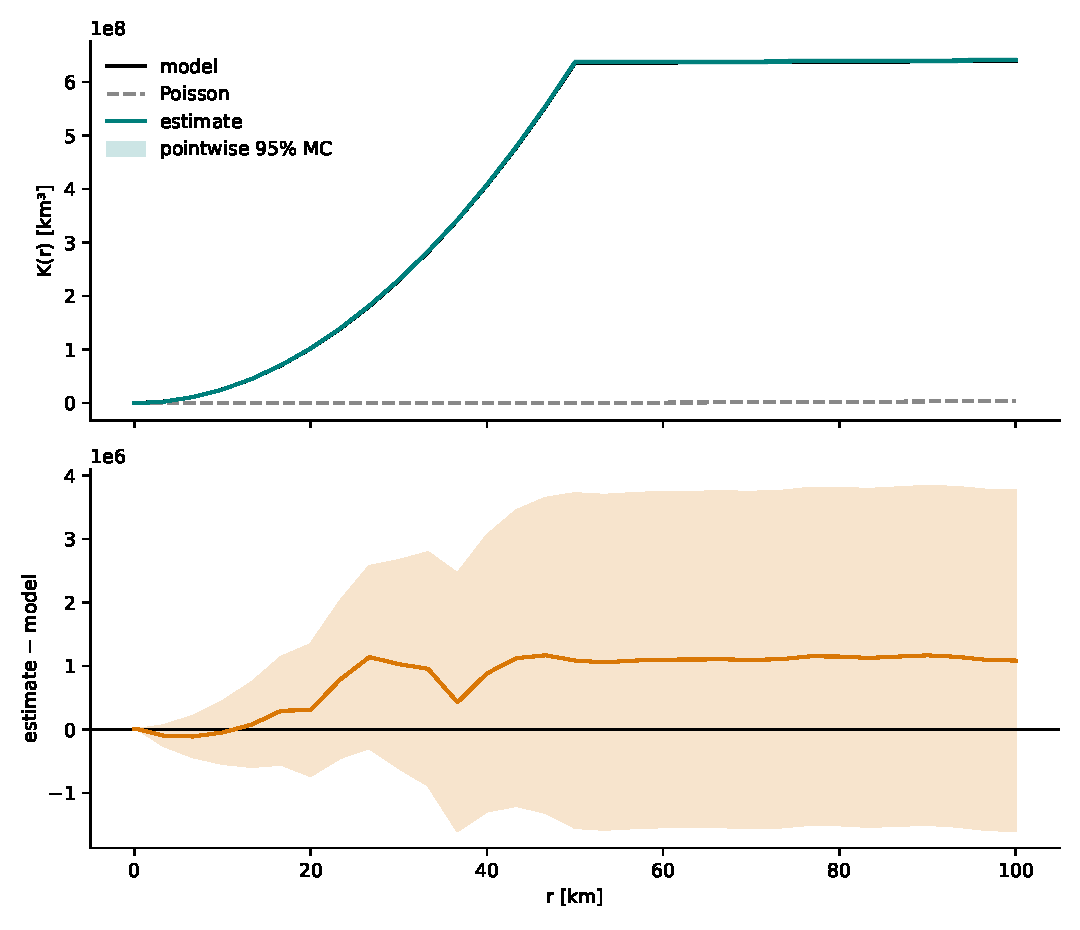
\includegraphics[width=0.83\textwidth]{figures/k_function.pdf}
 \caption{Translation-corrected three-dimensional $K$ estimate, analytical
 model curve and Poisson reference. Shading gives pointwise 95\% Monte Carlo
 intervals over independent realisations.}
 \label{fig:k-check}
\end{figure}

Across the six pair bins, the ratios of estimated to bin-averaged target $g_2$
range from $0.9991$ to $1.0061$. Across the four triangle bins the corresponding
$g_3$ ratios range from $0.9968$ to $1.0203$. Every pair and triangle target
lies in its pointwise interval. The compensated pair ratios range from $0.9995$
to $1.0055$, and the compensated triangle ratios from $0.9889$ to $1.0184$.
The independent geometric normalisers have relative standard errors below
$0.29\%$ for the pooled triangle bins; an independent lower-resolution
normaliser run changed their reciprocal averages by less than $0.44\%$.

\begin{figure}[htbp]
 \centering
 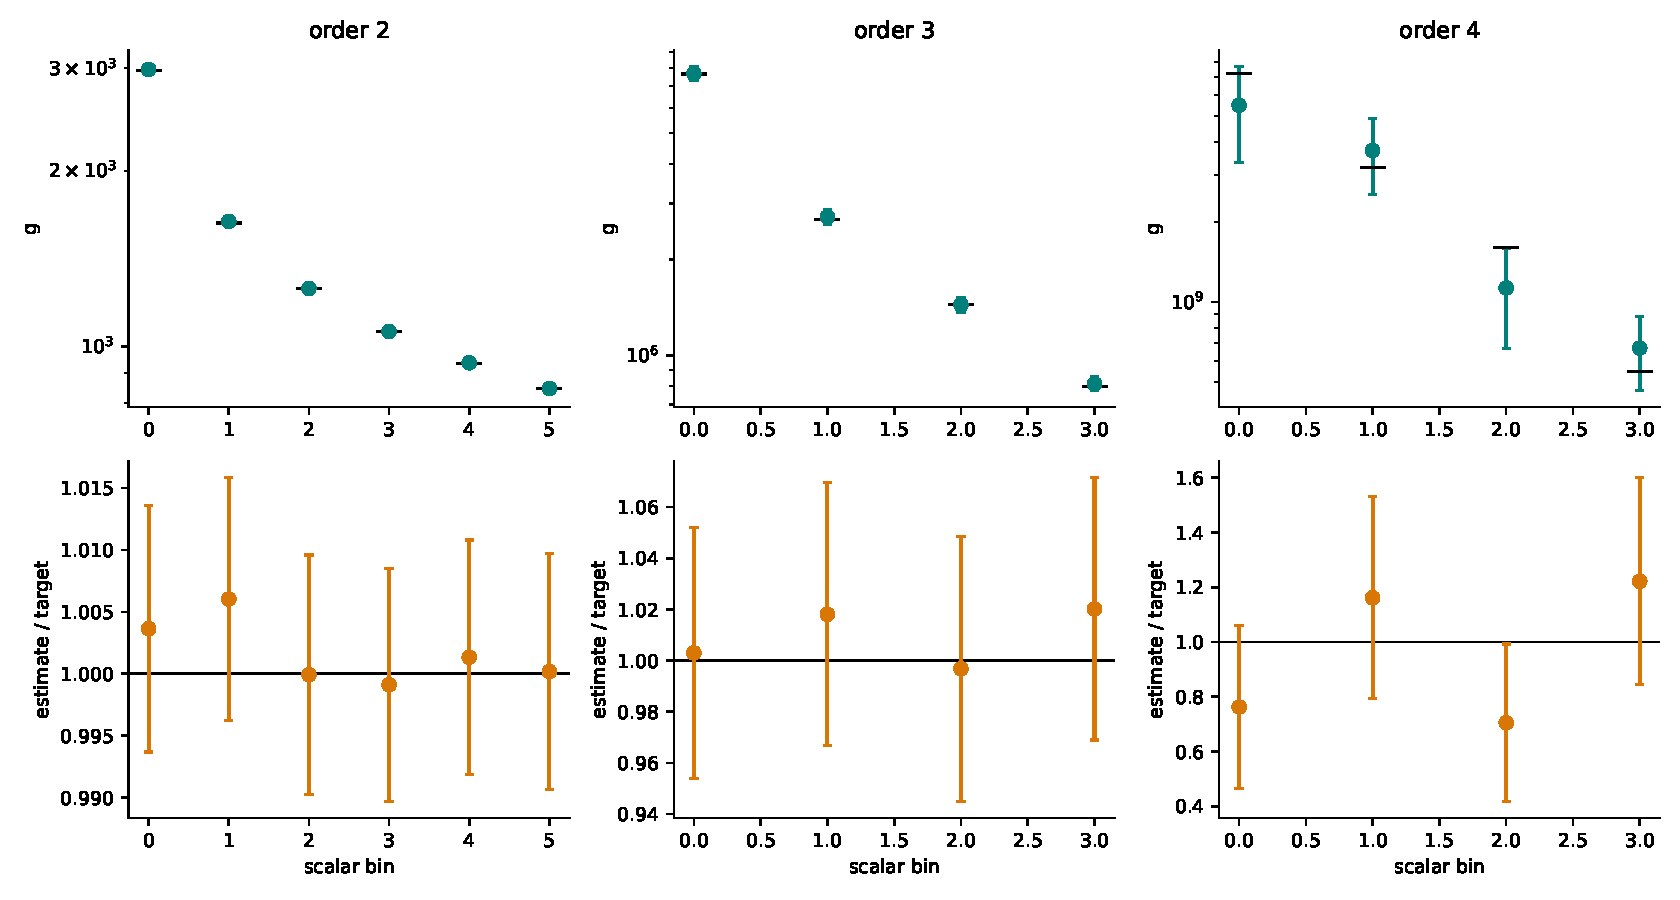
\includegraphics[width=\textwidth]{figures/correlations.pdf}
 \caption{Full correlation estimates against their integrated finite-bin
 reciprocal targets. The lower panels show estimate-to-target ratios. The
 fourth-order intervals are much wider because only 126 admissible
 tetrahedra were observed.}
 \label{fig:correlations}
\end{figure}

\begin{figure}[htbp]
 \centering
 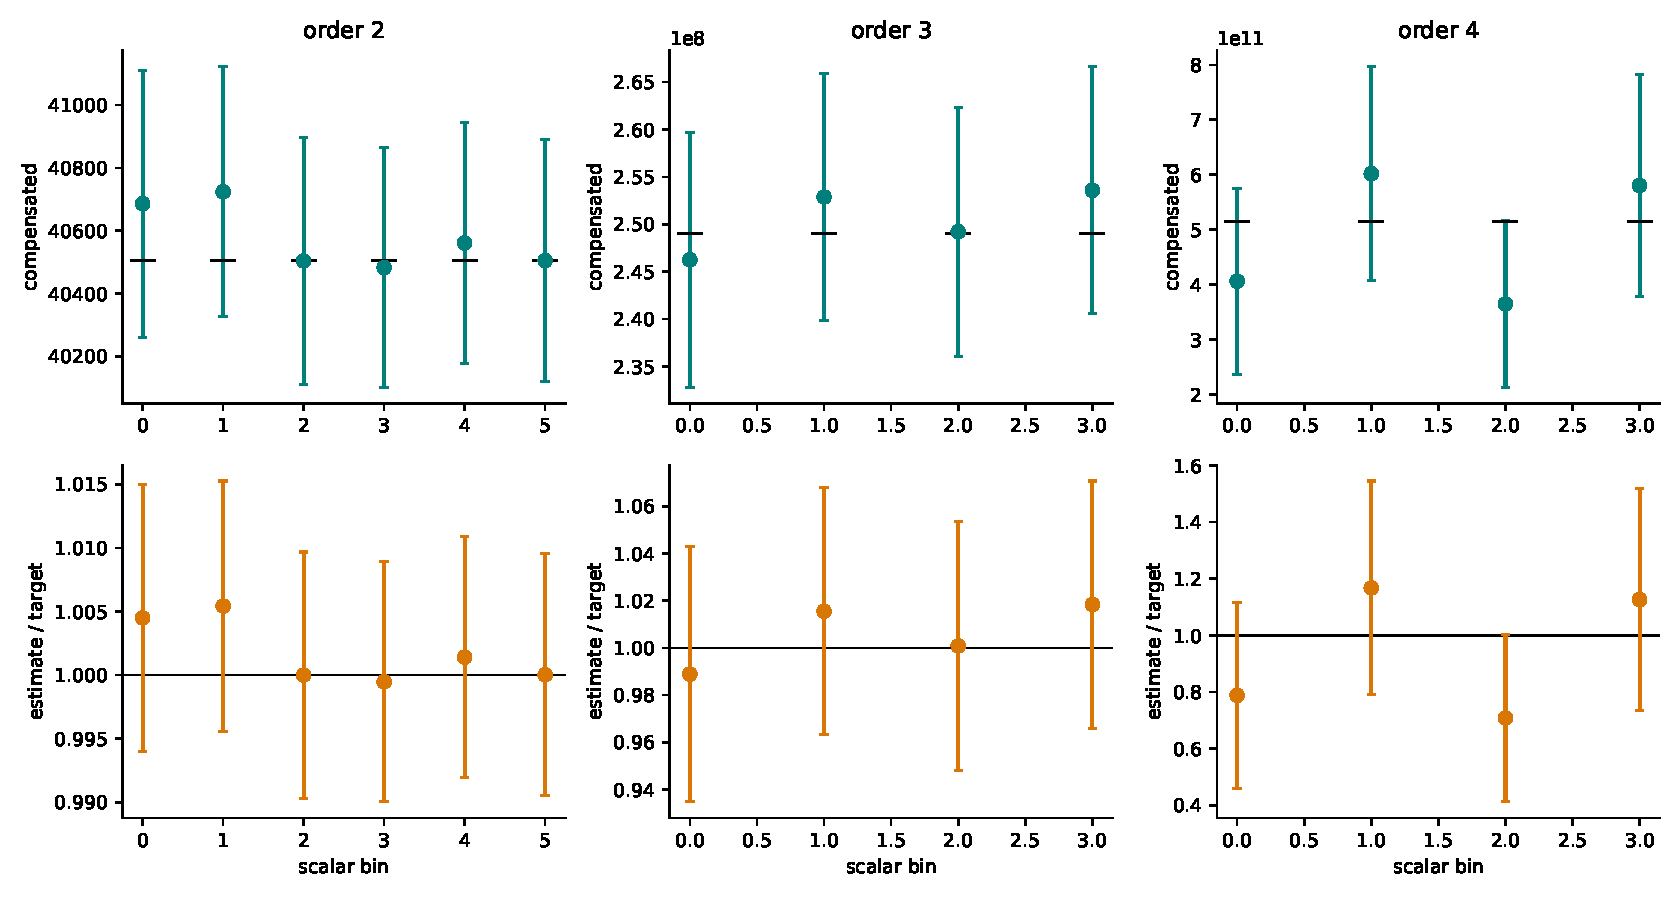
\includegraphics[width=\textwidth]{figures/compensated.pdf}
 \caption{Compensated estimates of $Dg_2$, $Ag_3$ and $Vg_4$ against the fixed
 constants $C_2,C_3,C_4$. Multiplying by the within-tuple geometric quantity,
 rather than a bin midpoint, preserves the exact finite-bin target.}
 \label{fig:compensated}
\end{figure}

Fourth order cannot support the same conclusion. Its four raw ratios are
$0.70$, $0.76$, $1.16$ and $1.22$ after ordering, with relative pointwise
half-widths between $28.8\%$ and $37.9\%$; one raw bin misses its target
interval. All four compensated intervals contain $C_4$, but their half-widths
reach $39.1\%$. The pooled fourth-order normalisers themselves are much more
stable, with relative standard errors below $0.63\%$. The limitation is the
number of observed tetrahedra, not geometric quadrature. These estimates are
inconclusive rather than evidence for or against the analytical identity.

The triangle shape and orientation strata show no resolved systematic
departure: all nonempty compensated intervals contain $C_3$, and the two
orientation groups have estimate-to-target ratios between $0.946$ and $1.069$.
One proposed triangle stratum is geometrically empty and is excluded:
$h_3/d_{\max}\leq0.3281$ implies
$A=d_{\max}h_3/2\leq215.10\,\mathrm{km}^2$, below that bin's lower edge
$223.24\,\mathrm{km}^2$. Fourth-order shape and orientation strata contain
between 0 and 40 tuples per bin and remain underpowered. The independent
normaliser check found no discrepancy larger than $1.82$ joint standard
errors, although one tiny fourth-order stratum changed in volume by $10.8\%$.

\begin{figure}[htbp]
 \centering
 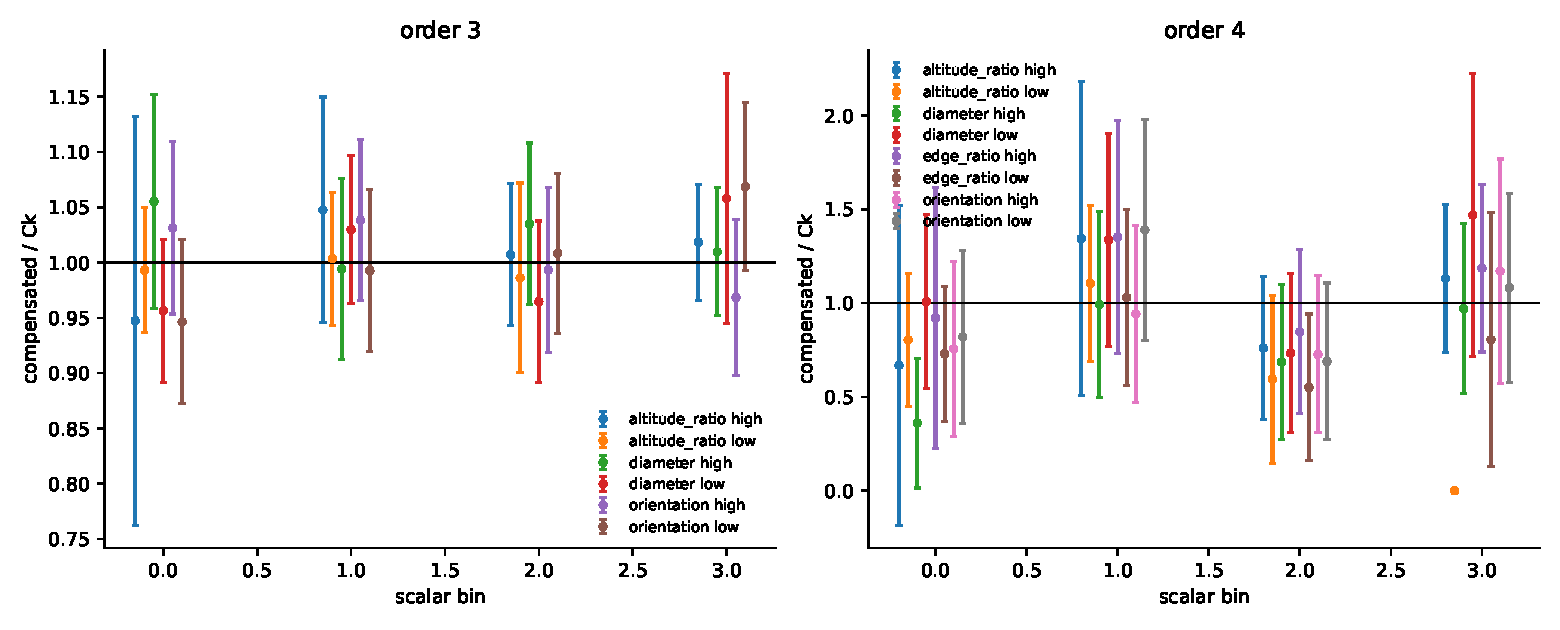
\includegraphics[width=0.9\textwidth]{figures/shape_strata.pdf}
 \caption{Compensated shape and orientation diagnostics. Triangle strata are
 informative except where explicitly sparse or geometrically empty;
 tetrahedron strata are shown to expose, not conceal, their low information.}
 \label{fig:shape-strata}
\end{figure}

Finally, the Poisson controls return correlations close to one at all three
orders. Every pooled Poisson interval contains one: their tuple counts are
$48{,}176$, $17{,}051$ and $7{,}006$ at orders two, three and four. This
separate test supports the ordered-tuple factors, geometric normalisation and
translation correction. It does not repair the sparse fourth-order
cluster-model estimate.

\begin{figure}[htbp]
 \centering
 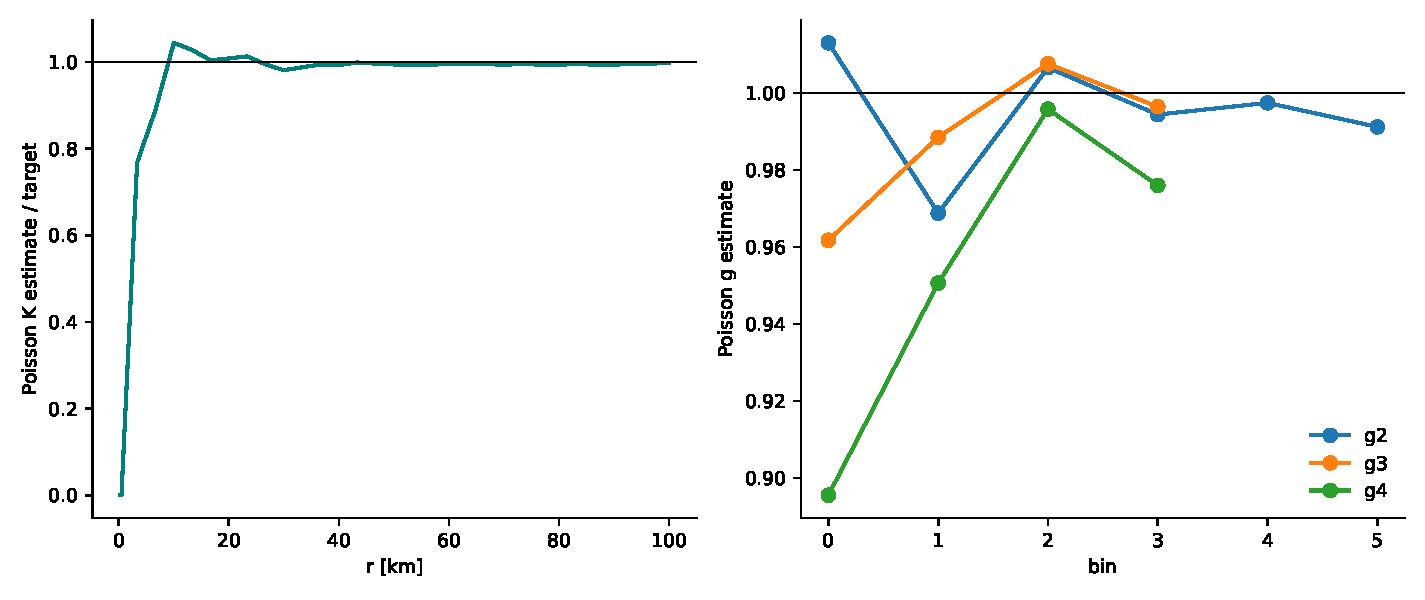
\includegraphics[width=0.85\textwidth]{figures/poisson_controls.pdf}
 \caption{Poisson controls for the $K$ and full-correlation estimators. The
 control intensity is deliberately higher than the witness intensity.}
 \label{fig:poisson-controls}
\end{figure}

All intervals in this section are the pointwise normal intervals defined in
Appendix~\ref{app:estimators}: the relevant mean plus or minus $1.95996$ times
its realisation-level standard error. They are not simultaneous bands or
prediction envelopes. Geometric-normaliser uncertainty is recorded separately
and combined diagnostically, rather than hidden in the realisation-level
standard error.
The normal approximation is particularly rough for the rare fourth-order
contributions and is reported only as a transparent measure of the attained
underpower.
Finite bins and finitely many shape strata do not prove pointwise identities
on a continuum. Their role is to test the implementation against the theorem.
